\section{Motivation}
\label{sec:motivation}

Let us consider the following motivating example in Figure \ref{fig:motiv} where different classification accuracy has been obtained every time machine learning model has been trained on the same dataset  \footnote{https://stackoverflow.com/questions/55775450/different-classification-accuracy-every-time-i-train-models-on-the-same-dataset}. 
\begin{figure}[h]
	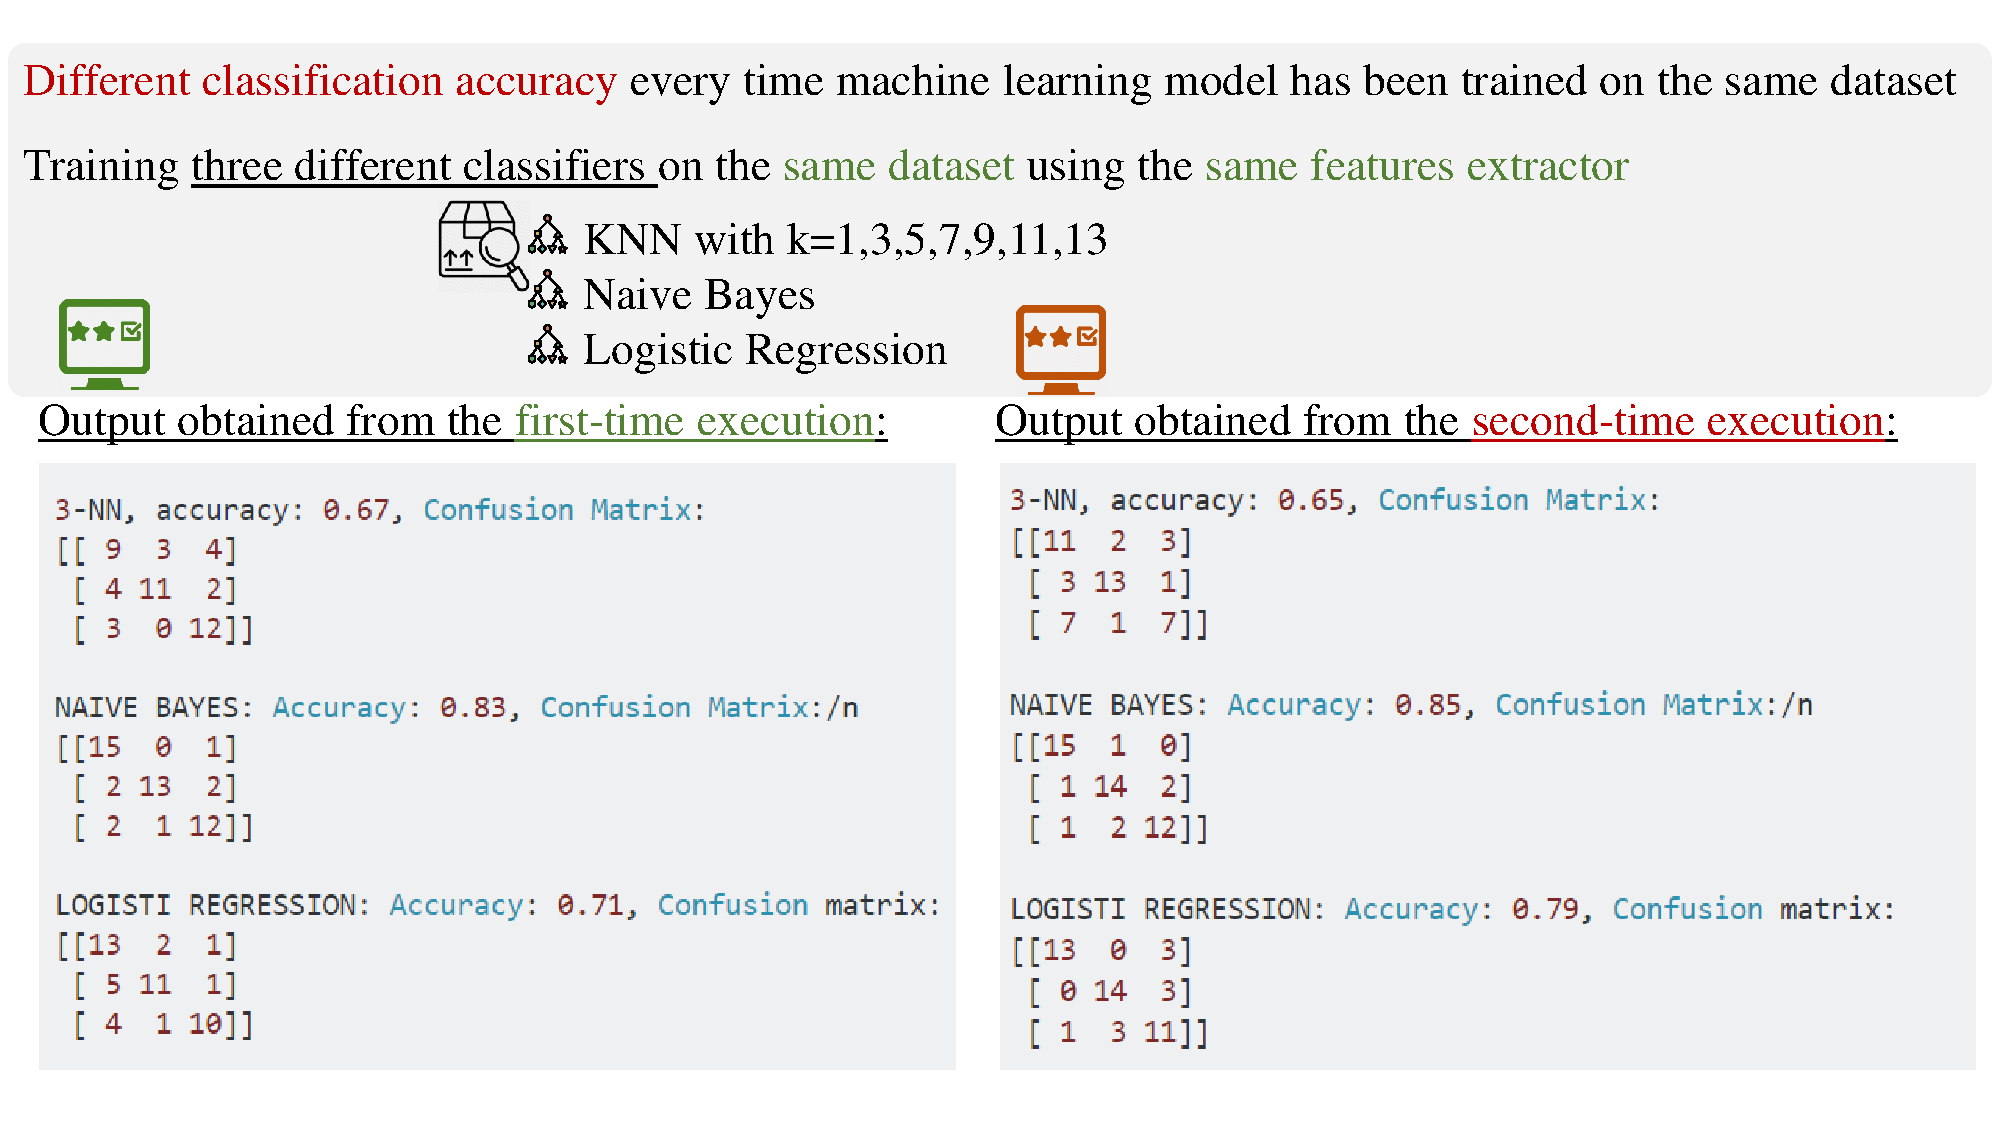
\includegraphics[width=\linewidth]{motivfigure.pdf}
	\caption{Motivating example of accountable assertion to interpret accuracy for accountable machine learning classifier}
	\label{fig:motiv}
	%\vspace{15pt}
\end{figure}
Here, three different classifiers e.g., k-nearest neighbors (k=1,3,5,7,9,11,13), Naive Bayes and Logistic Regression have been implemented on the same dataset using the same features extractor for comparing the accuracies to determine which classifier is better on the dataset. However, every time these models have been trained i.e., the whole code has been re-executed on the same dataset, different values of accuracy for each model has been obtained as illustrated in the Figure \ref{fig:motiv}. In this case, how we can interpret the accuracy or how the classifier can be accountable in terms of definite accuracy for each model? That is why we are motivated to propose an accountable assertion to interpret accuracy for accountable machine learning classifier.  



%\small
%\begin{lstlisting}[language=Python, caption=Motivating example of model verification to interpret accuracy for accountable ML]
%//The first time execution of a CNN code gives this output:
%3-NN, accuracy: 0.67, Confusion Matrix:
%[[ 9  3  4]
%[ 4 11  2]
%[ 3  0 12]]
%
%NAIVE BAYES: Accuracy: 0.83, Confusion Matrix:/n
%[[15  0  1]
%[ 2 13  2]
%[ 2  1 12]]
%
%LOGISTIC REGRESSION: Accuracy: 0.71, Confusion matrix:
%[[13  2  1]
%[ 5 11  1]
%[ 4  1 10]]
%
%\\ The second time execution of the same code returns:
%3-NN, accuracy: 0.65, Confusion Matrix:
%[[11  2  3]
%[ 3 13  1]
%[ 7  1  7]]
%
%NAIVE BAYES: Accuracy: 0.85, Confusion Matrix:/n
%[[15  1  0]
%[ 1 14  2]
%[ 1  2 12]]
%
%LOGISTIC REGRESSION: Accuracy: 0.79, Confusion matrix:
%[[13  0  3]
%[ 0 14  3]
%[ 1  3 11]]
%\end{lstlisting}
